\section{Theoretical Background}
\label{sec:theory}

\subsection{Convolutional Neural Networks}
\label{subsec:cnn}

The application of CNNs in climate science has yielded several notable contributions. According to the sources provided, CNNs have excelled at extracting patterns and features from spatial data such as satellite imagery, radar data, and climate model outputs. This capability has enabled researchers to better understand and predict complex atmospheric and oceanic phenomena. For instance, CNNs have been employed to detect and localize extreme weather events from satellite data, enhancing early warning systems and disaster response efforts. Furthermore, CNNs have improved the ability to identify forced climate patterns and disentangle natural variability from human-induced climate change signals, advancing our understanding of climate dynamics and informing mitigation strategies.


Convolutional neural networks (CNNs) are a type of deep learning architecture inspired by the visual cortex of animals. They are designed to efficiently capture spatial and temporal dependencies in data through the use of learnable filters and hierarchical feature representations. Through the use of convolutional layers instead of fully connected layers, the architecture is able to preserve the spatial structure of the input data, making it particularly well-suited for image and video data. This approach not only simplifies pattern detection but also implies a reduction in the number of parameters, which minimizes the necessary computational resources.

Application of CNNs in climate science has yielded several notable contributions, including the reconstruction of the El Nino event of 1877 by Kadow et al. despite extremely limited data availability. \cite{kadow2020} 


\subsubsection*{Convolutional Layer}
\begin{figure}
    \centering
    \animategraphics[loop,autoplay,width=400pt]{1}{resources/images/convolution_gif/convolution_kernel-}{0}{15}
    \caption{How a convolution operation works. \cite{datahacker}}
    \label{fig:convolution_operation}
\end{figure}

The convolutional layer is the driver for feature mapping in a CNN. It applies a convolution operation shown in \autoref{fig:convolution_operation} to the input data. The operation is done element by element while sliding a filter (also called kernel) over the input data such that situations, where the filter overflows the input data ranges, are avoided or taken care of. On each step, the Frobenius Product between the kernel and the submatrix given by the current position and the kernel dimension is calculated and noted in the output matrix. The parameters in the kernel matrix are chosen in such a way that the Frobenius Product is maximized when the kernel is over a feature that the kernel is supposed to detect. In \autoref{fig:convolution_operation} the kernel for example is a vertical edge detector, meaning it will output a high amount (positive or negative) when the horizontal gradient in the input data submatrix has a high absolute value. This result is rather trivial, as a positive horizontal gradient as seen in the upper-left 3x3 submatrix of the example leads to a right column that when negatively weighted overweights the positive-weighted left column and thus the output for the upper-left 3x3 submatrix is negative. Conversely, a Fresenius product of the upper-right 3x3 submatrix with the kernel returns a positive value, hinting at a negative horizontal gradient in the input data. The result of such a convolution can be observed in \autoref{fig:edge_detection}.

In the context of weather data, the convolutional layer can be used to detect any weather patterns not just edges and the kernel itself can be learned by the network.

\begin{figure}
    \centering
    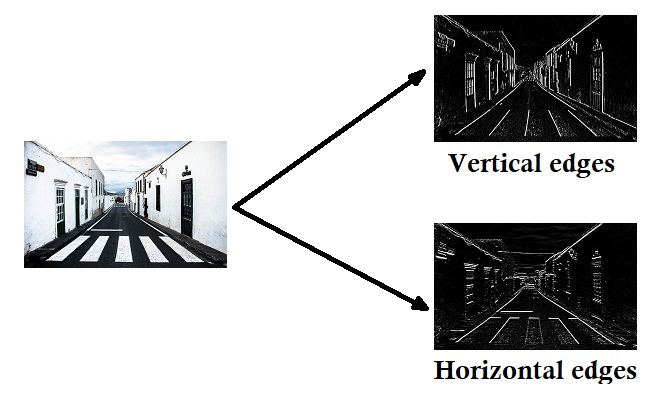
\includegraphics[width=250px]{resources/images/edge_detection.jpeg}
    \caption{Example of edge detection with a convolutional kernel. \cite{datahacker}}
    \label{fig:edge_detection}
\end{figure}

\subsubsection*{Activation Function}

\subsubsection*{Pooling Layer}

The exact position of a low-level feature in the input data is not so important when it comes to detecting high-level features,
it is more important to recognize if a feature is present at all in certain spatial areas of the input data or not.
Thus scaling down the resolution of the matrix by combining every 2x2 submatrix into one value can be beneficial.
It is most commonly aggregated by taking the maximum value of the submatrix because it works for the mentioned purpose to detect if a feature is present in the area of the submatrix or not. While the convolution layer depending on how the convolution is processed near the borders of the input data reduces the dimensionality of the input data just slightly or not at all, the pooling reduces the dimensionality drastically. So after a 2x2 pooling operation, the output matrix is only a quarter of the size of the input matrix.

\begin{figure}
    \begin{subfigure}{1\textwidth}
        \centering
        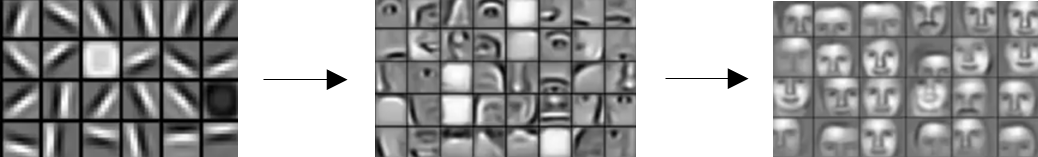
\includegraphics[width=0.9\textwidth]{resources/images/abstraction.png}
        \caption{Low-level features are combined into high-level features.}
        \label{fig:abstraction}
    \end{subfigure}
    \vspace{0.5cm}
    \begin{subfigure}{0.7\textwidth}
        \centering
        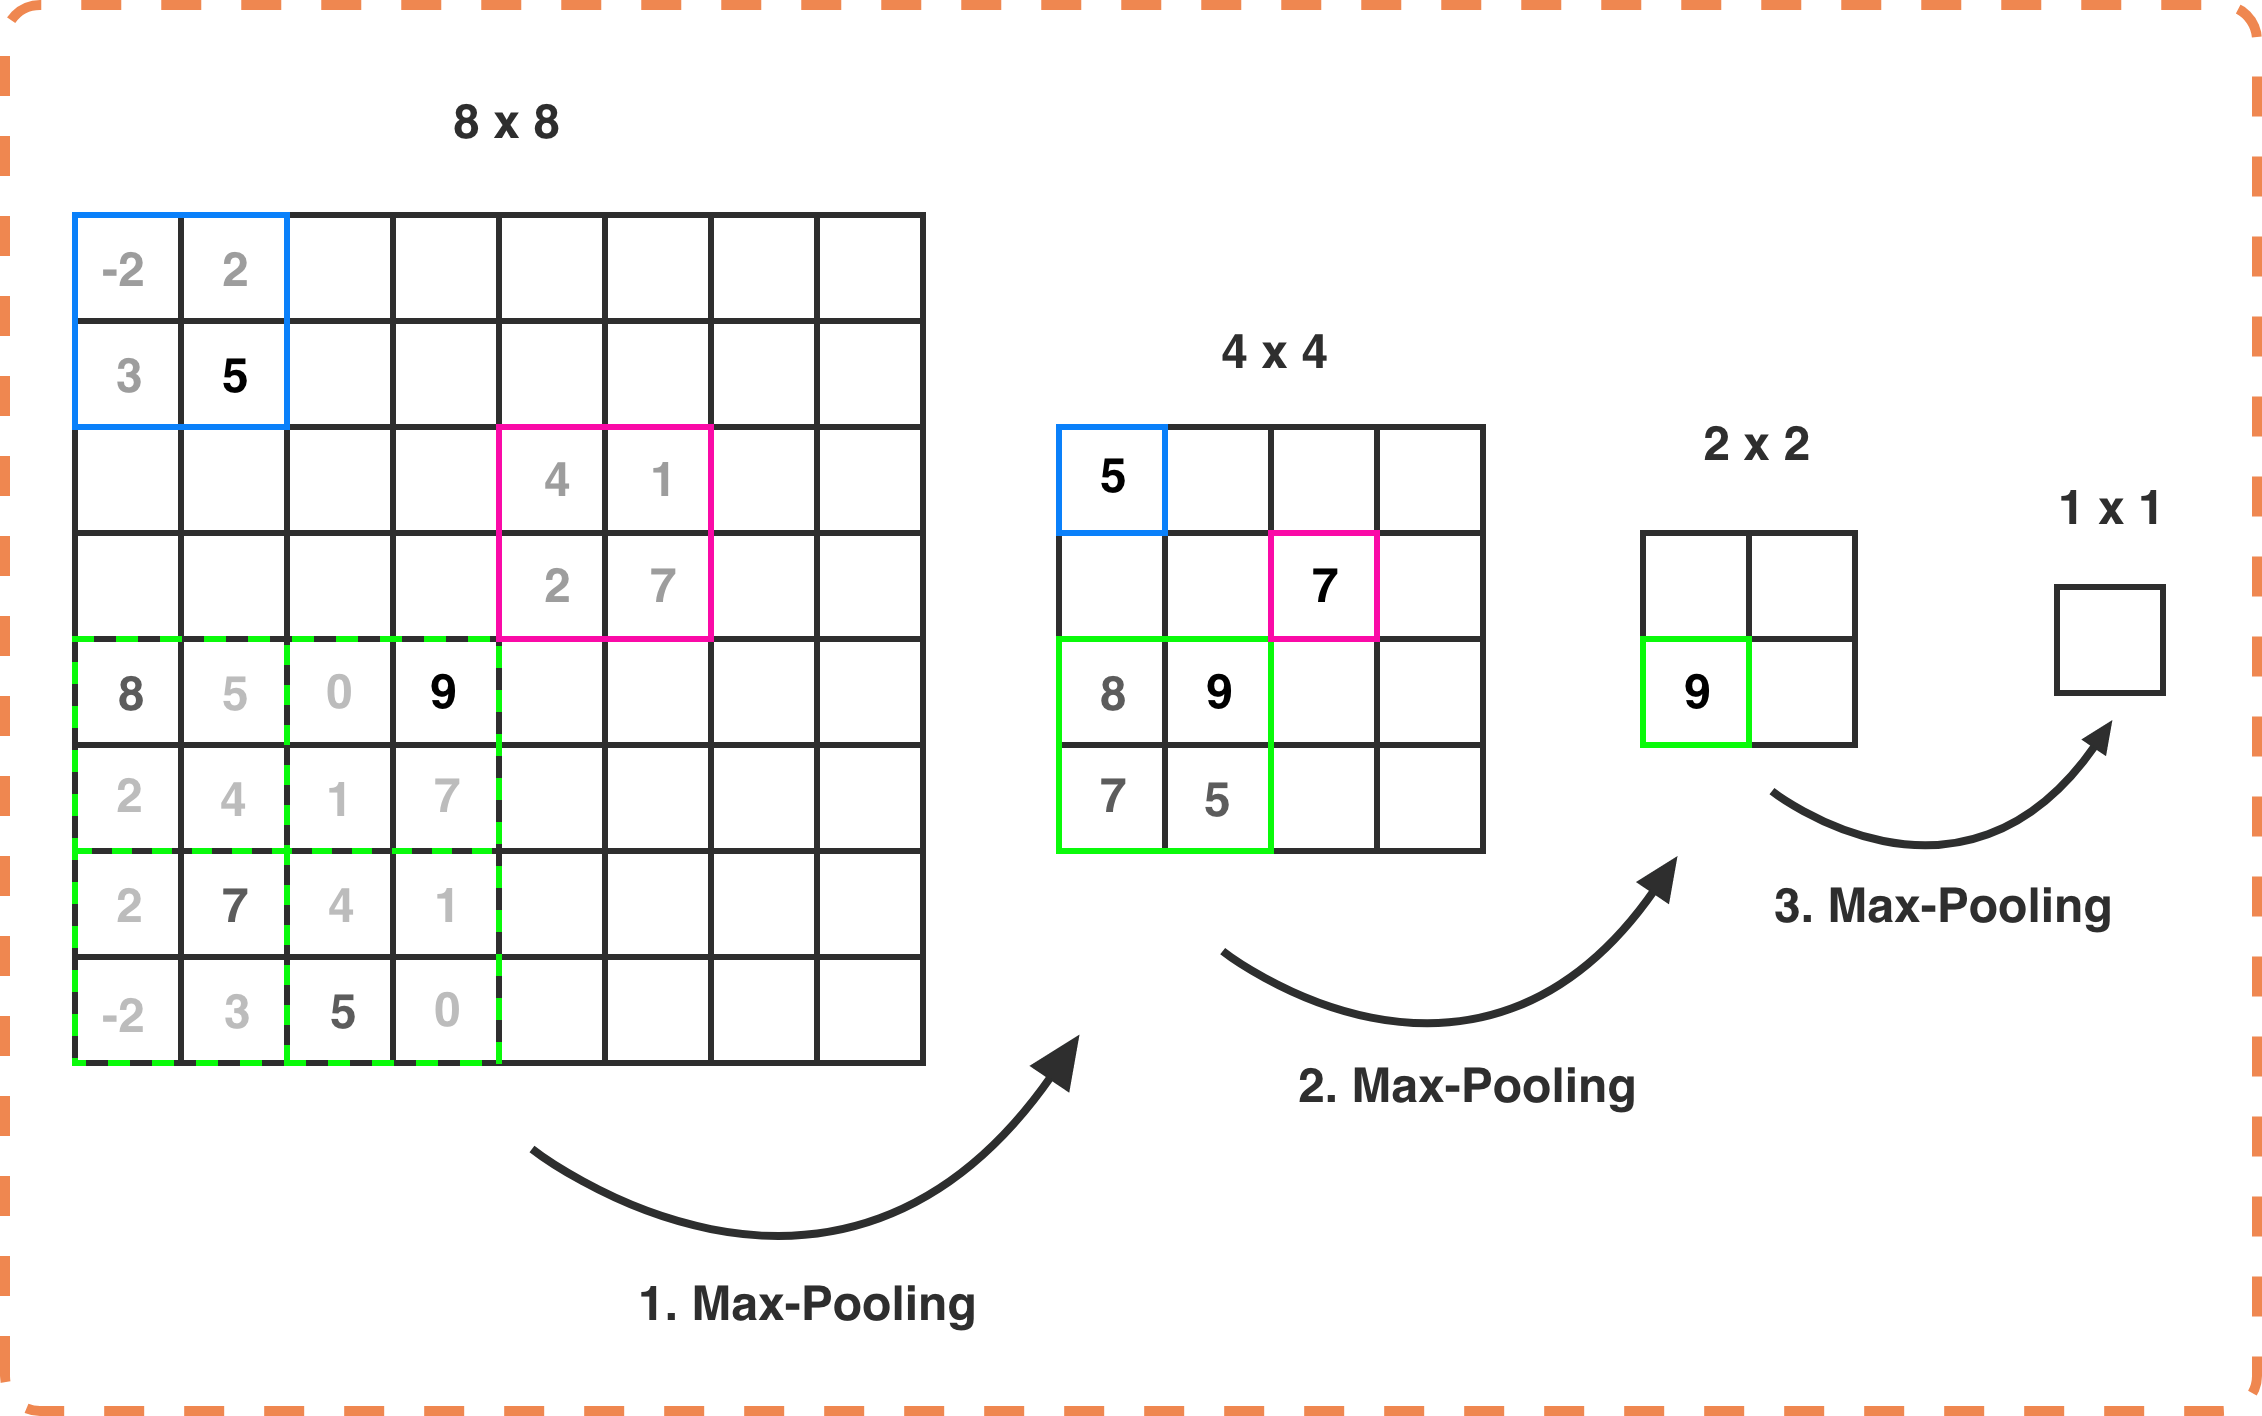
\includegraphics[width=0.9\textwidth]{resources/images/max_pooling.png}
        \caption{Illustration of 3 max pooling layers.}
        \label{fig:max_pooling}
    \end{subfigure}
    \begin{subfigure}{0.25\textwidth}
        \centering
        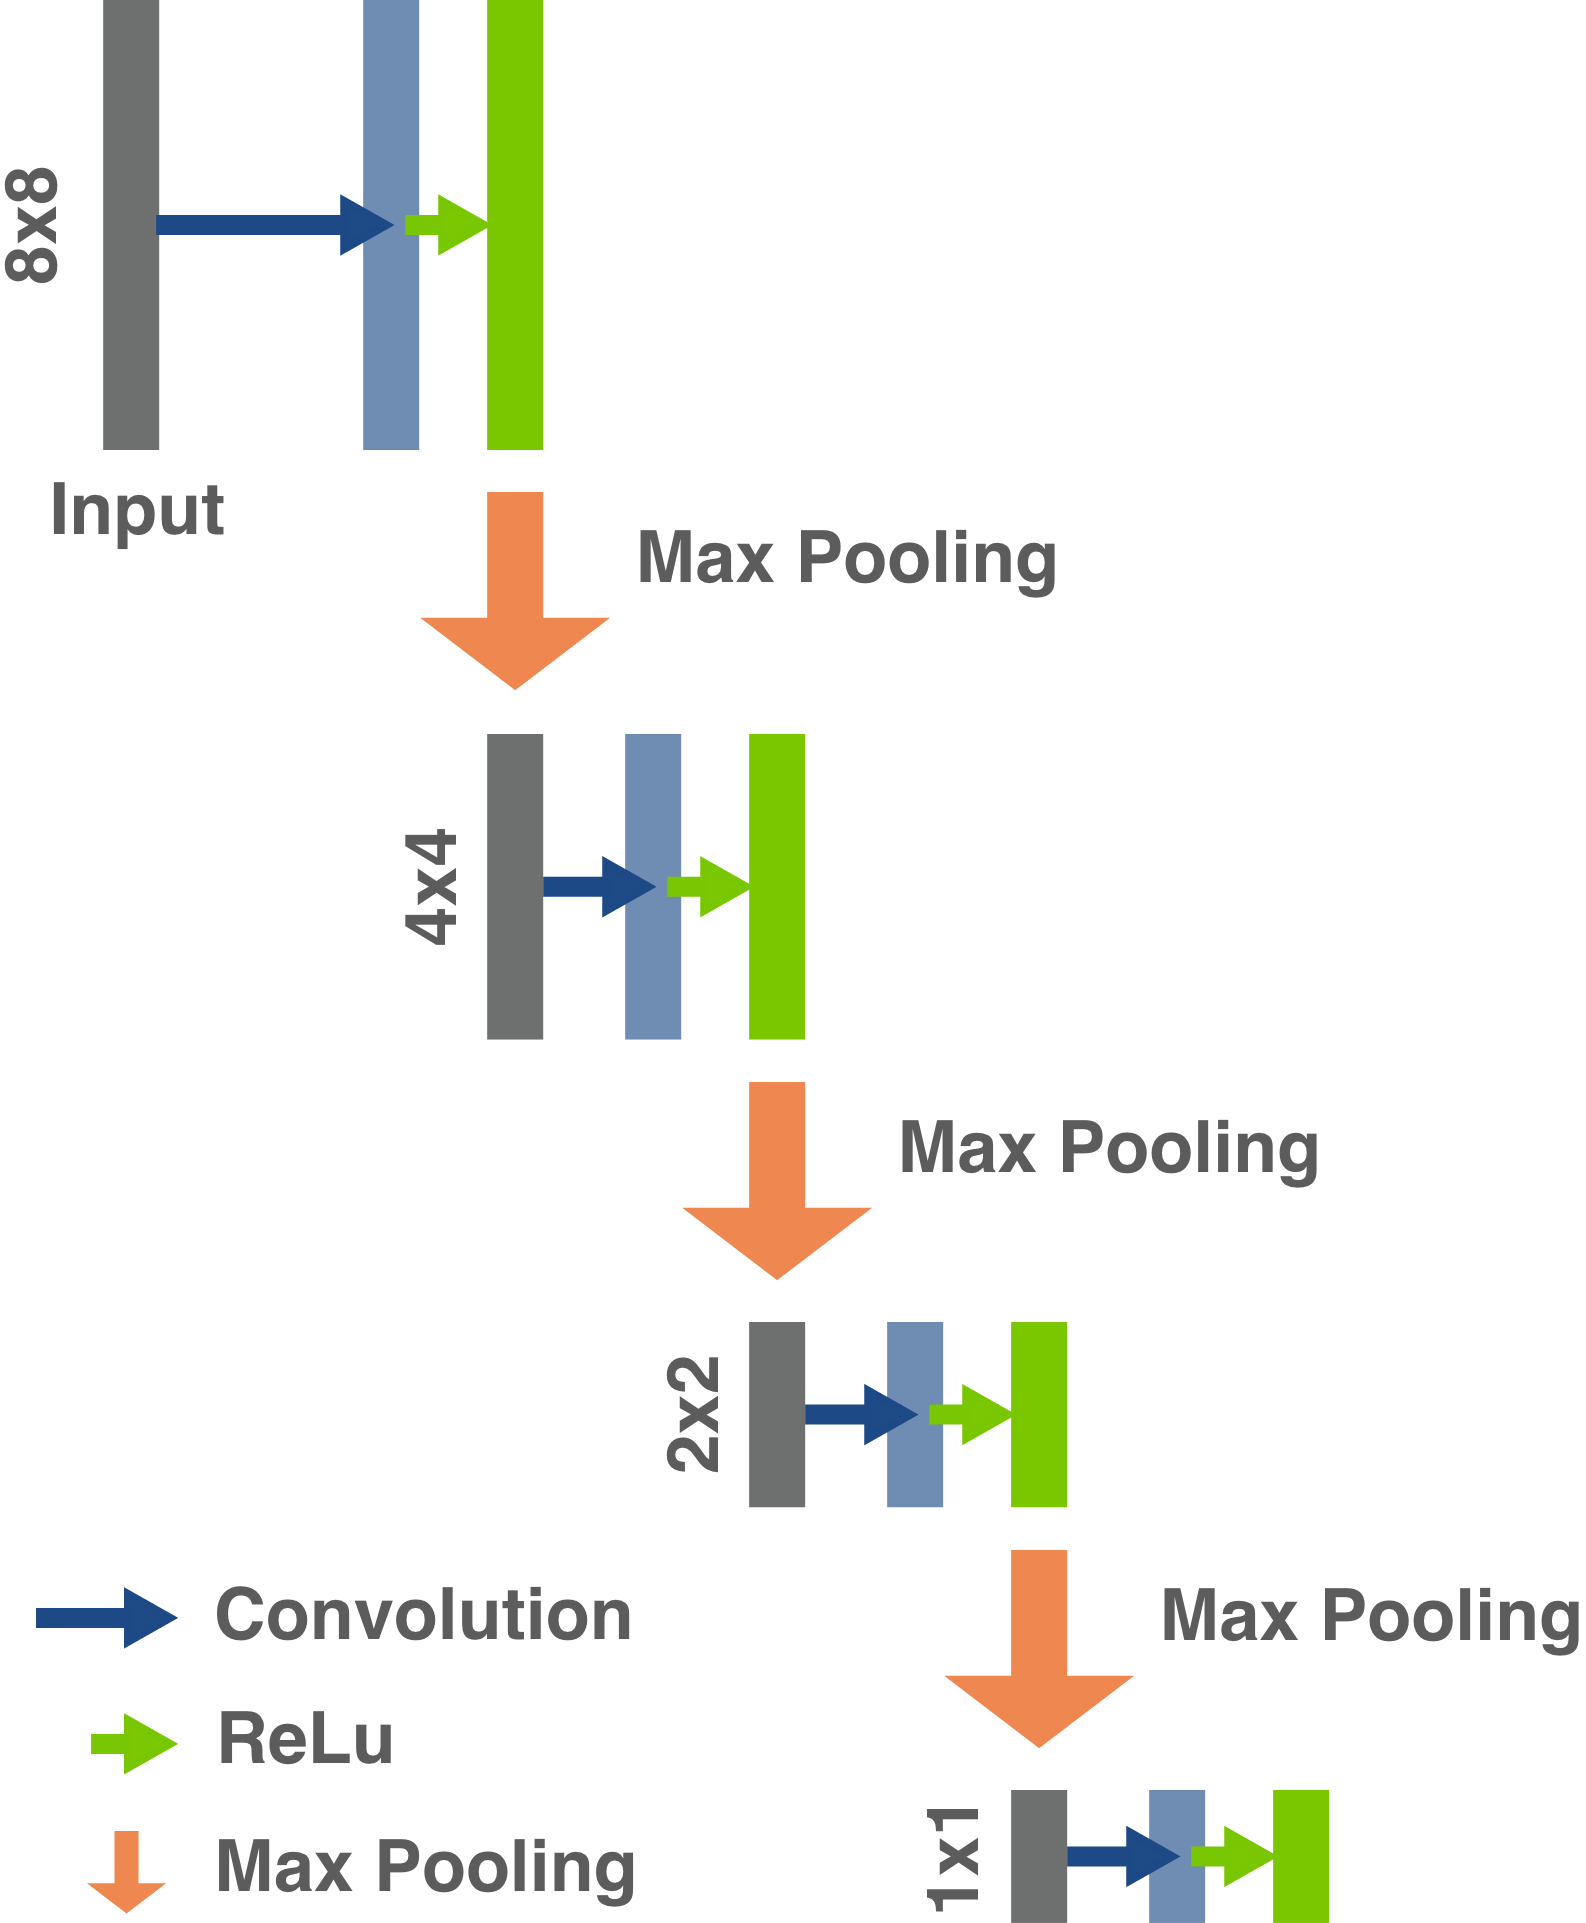
\includegraphics[width=0.9\textwidth]{resources/images/encoder_architecture.png}
        \caption{How Convolutional layers and pooling layers alternate}
        \label{fig:encoder_architecture}
    \end{subfigure}
    \caption{Abstraction in the encoding part of a CNN.}
\end{figure}


For the 8x8 grid cells of the ERA5 data, that is used as input in the laid out approach (see \autoref{subsec:data_preprocessing}), the architecture of the CNN could include a maximum of 3 pooling layers, reducing the input data to a 1x1 matrix as seen in \autoref{fig:max_pooling}. \autoref{fig:max_pooling} just illustrates the downsampling of the data, in the actual architecture pooling layers always follow convolutional layers and are never applied directly after each other as seen in \autoref{fig:encoder_architecture}. 

\subsubsection*{Upscaling Layer}

\subsubsection*{Skip Connections}

\subsubsection*{Supervised Learning}

\subsection{Reanalysis - ERA5}

Atmospheric reanalysis is a numerical method to estimate the state of the atmosphere at any given time, opposing missing measurements. The method is based on a complex numerical model, simulating the physical rules of the atmosphere. As any numerical model, it has degrees of freedoms, allowing for adjustments of parameters, which are chosen in such a way that the model output is matching the actual measurements where ever they are available in space and time.

The ERA5 reanalysis is a product of the European Centre for Medium-Range Weather Forecasts (ECMWF) and is the fifth generation of the ERA reanalysis series. It provides atmospheric reanalysis data globaly at the earth surface as well as on different pressure levels. The data is available from 1940 to present and has a temporal resolution of 1 hour. The spatial resolution of the data is 0.25 degrees, which is approximately 28 km at the equator, given that the equator has a length of 40,075 km. The data is available for a wide range of variables, including temperature, precipitation, wind speed, and many more. 